\chapter{Equity Markets}
\renewcommand{\thesection}{3.1 - 3.2}
\section{Introduction and Key Concepts}
\setcounter{section}{2}
\renewcommand{\thesection}{\arabic{chapter}.\arabic{section}}

\begin{definitionbox}{Equity}
    The value of the ownership stake in a firm– the residual claim on the firm's assets after all other claims have been paid.
\end{definitionbox}

\begin{definitionbox}{Shares}
    Shares represent how the equity stake is divided. As a shareholder, you have right to claim portion of the company's profits, and control over the company's decisions.
\end{definitionbox}

These terms are sometimes used interchangeably, although they have slight differences.

\begin{itemize}
    \item Companies decide on the \textbf{allocation of profits} between reinvestment in the business and distribution as dividends, which are \textbf{distributed proportionately} to shareholders based on their shareholdings.
    \item The corporate structure and shareholder rights are established through \textbf{articles of association} (UK) or \textbf{articles of incorporation} (US), filed with Companies House in the UK or with the Secretary of State's office in the respective state in the US.
    \item Articles also delineate shareholder rights, including \textbf{voting and influence over management decisions}.
    \item As a company expands, it may \textbf{issue more shares to raise capital}, thus increasing the number of shareholders and shares in circulation.
    \item Some companies may decide to hold an \textbf{Initial Public Offering (IPO)}, which involves listing the company on a stock exchange, publicly.
    \item Shareholders exert control through a \textbf{voting process} in important company decisions such as issuing shares, debt management, and significant corporate actions like mergers and acquisitions.
    \item In the US, public companies are mandated to hold an \textbf{Annual General Meeting (AGM)}, where shareholders vote on crucial matters including the board of directors and executive compensation.
    \item There is a growing trend of shareholders influencing a company's \textbf{social and environmental practices}, asserting their rights and preferences in corporate governance.
    \item Active participation in voting and discussions at shareholder meetings helps \textbf{shape the company's direction and governance}.
\end{itemize}

\begin{enumerate}
    \item \textbf{Ownership vs. Creditship}
    \begin{itemize}
        \item Shares represent ownership in a company, providing rights to profits and decision-making.
        \item Bonds are debt obligations; bondholders are creditors, lending money without ownership rights.
        \item Shareholders have voting rights and participate in decisions like elections and mergers.
        \item Bondholders typically do not have voting rights, reflecting their role as lenders.
    \end{itemize}

    \item \textbf{Tax Treatment}
    \begin{itemize}
        \item Interest payments to bondholders are tax-deductible as business expenses, reducing taxable income.
        \item Dividends to shareholders are paid from after-tax profits and are not deductible.
    \end{itemize}

    \item \textbf{Priority of Payments or Seniority}
    \begin{itemize}
        \item In bankruptcy, bondholders have higher claim priority on assets than shareholders.
        \item Shareholders are residual claimants, receiving assets only after all creditors are paid.
    \end{itemize}

    \item \textbf{Risk and Return}
    \begin{itemize}
        \item Shares offer potential high returns but come with higher risks, including losses.
        \item Bonds provide stable returns through interest payments and principal repayment on maturity.
    \end{itemize}

    \item \textbf{Credit Risk}
    \begin{itemize}
        \item Bondholders have legal recourse (the right to take legal action) in defaults, able to reclaim their investment.
        \item Shareholders cannot demand dividends and must wait for company profitability to improve.
    \end{itemize}
\end{enumerate}


\begin{examplebox}{True or False?}

\begin{figure}[H] 
        \footnotesize
        \centering
        \begin{tabular}{|p{2.8cm}|p{2.8cm}|p{2.8cm}|p{2.8cm}|p{2.8cm}|}          
        \hline
        \textbf{Question} & \textbf{Option 1} & \textbf{Option 2} & \textbf{Option 3} & \textbf{Option 4} \\
        \hline
        Which of the following statements correctly relates to shares or shareholders? & 
        Ordinary shares represent the equity share capital of the firm. \textbf{True} & 
        Ordinary shareholders are the last in the queue to have their claims met. \textbf{True} & 
        Shareholders have the right to exercise control over the company. \textbf{True}& 
        The shareholder will always receive back the original capital invested. \textbf{False} \\
        \hline
        Which of the following statements best describe a company’s debt capital holders? & 
        They will always receive back their original capital. \textbf{False} & 
        They have no formal control. \textbf{True}& 
        They receive interest and may recover capital. \textbf{True} & 
        They have an equity interest in the company. \textbf{False}\\
        \hline
        Which of the following statements best describe the costs of equity when compared with debt capital? & 
        Equity finance is less expensive for companies. \textbf{False} & 
        Investing via debt finance is less risky for investors. \textbf{True}& 
        Investing via equity finance is less risky for investors. \textbf{False}& 
        Debt finance is less expensive for companies. \textbf{True}\\
        \hline
        Which of the following statements accurately describe the taxation of dividends and loans? & 
        Dividends are paid out of after-tax earnings. \textbf{True} & 
        The company will generally prefer equity finance since it is more tax-efficient. \textbf{False}& 
        Dividends can be used to reduce a firm’s taxable profits.\textbf{False} & 
        Interest payments on a loan are tax deductible. \textbf{True} \\
        \hline
        \end{tabular}
        \caption{Comparison of Shareholder and Debt Holder Attributes}
        \label{table:share_debt}

\end{figure}

\end{examplebox}



\section{Introduction to Equity Valuation}
There are three primary approaches to valuing shares:

\begin{itemize}
    \item \textbf{Dividend Discount Model (DDM):} 
    \begin{itemize}
        \item This model takes a directly estimates the present value of expected dividends. 
        \item The value of a share is derived from the present value of anticipated dividend payments. 
        \item Since dividends are uncertain and not predetermined, their expected values are considered.
    \end{itemize}
    
    \item \textbf{Discounted Cash Flow (DCF) Modelling:} 
    \begin{itemize}
        \item Widely employed by equity analysts, this indirect approach focuses on valuing the entire firm first. 
        \item This valuation is determined by discounting the expected future cash flows generated by the company. 
        \item After valuing the enterprise, all liabilities, such as debts and leases, are deducted from the enterprise value. 
        \item The residual amount, attributed to the shareholders, is then divided by the number of shares to provide the value per share. 
    \end{itemize}
    
    \item \textbf{Multiples Approach:} 
    \begin{itemize}
        \item This method estimates the value of a company by comparing it to similar companies in the market using financial ratios or multiples, such as the price-to-earnings ratio (P/E) or the enterprise value-to-EBITDA (EV/EBITDA). 
        \item Multiples valuation is a quick and straightforward approach, relying on market-based data and the performance of similar companies.
    \end{itemize}
\end{itemize}


\subsection*{Dividend Discount Model}
\begin{definitionbox}{Dividend Discount Model}
\textbf{Assumptions:}
\begin{enumerate}
    \item \textbf{Zero-Growth Dividend Model: }\\Assume dividend stream is constant over time, like a zero-growth perpetuity. Assume first dividend payment is received one year from now.
    \begin{equation}
        P_0 \text{ (current price of the stock)}= \frac{D_1 \text{ (expected dividend payment)}}{r \text{ (required rate of return on equity or cost of equity)}}
    \end{equation}
    \item \textbf{Constant-Growth Dividend Model (Gordon Growth Model): }\\Assume dividend stream will grow at a constant rate indefinitely into the future, like a growing perpetuity.
    \begin{equation}
        P_0 \text{ (current price of the stock)}= \frac{D_1 \text{ (the expected payment at the end of the upcoming period)}}{r \text{ (cost of equity)} - g \text{( the growth rate of dividends)}}
    \end{equation}
    \item \textbf{Multi-Period Dividend Model (Dividend Discount Model for Multiple Periods): }\\Assumption (involving having information about dividends for the next $n$ years) that either the dividend stream remains constant or grows at a constant rate. Thus, the value of the stock is calculated as such
    \begin{equation}
        P_0 = \frac{D_1}{(1+r)} + \frac{D_2}{(1+r)^2} + \ldots + \frac{D_n}{1+r^n} + \frac{\frac{D_n \times (1+g)}{(r-g)}}{(1+r)^n}
    \end{equation}
\end{enumerate}

\textbf{Do note that these models only price a stock based on dividend cash flows and do not consider other factors like capital gains, etc.}

\end{definitionbox}

\begin{examplebox}{Bits 'n' Pieces Stock Return}
    Bits ‘n’ Pieces pays a constant annual dividend of £0.50 a share. The market price of the stock is £5.41 today. What is the rate of return on this stock?
    
    The rate of return can be calculated using the formula:
    \begin{align*}
        r_E &= \frac{\text{Div}}{P_0} \\
        &= \frac{0.50}{5.41} \\
        &= 0.09242 \\
        &= 9.24\%
    \end{align*}
    Therefore, the rate of return on this stock is 9.24\%.
\end{examplebox}

\begin{examplebox}{JLE Inc Stock Valuation}
    JLE, Inc. just paid its annual dividend of £1.10 a share. JLE’s policy is to increase the dividend by 2\% annually. How much are you willing to pay today for a share of this stock if you require an 11\% rate of return?
    
    The present value of the stock can be calculated as:
    \begin{align*}
        P_0 &= \frac{Div_1}{r_E - g} = \frac{Div_0 \times (1 + g)}{r_E - g} \\
        &= \frac{1.10 \times (1 + 0.02)}{0.11 - 0.02} \\
        &= \frac{1.122}{0.09} \\
        &= 12.46667 \\
        &\approx £12.47
    \end{align*}
    Hence, you would be willing to pay approximately £12.47 for a share of this stock.
\end{examplebox}

\begin{examplebox}{Isaac's Shoes Stock Valuation}
    Isaac’s Shoes just announced that it will commence paying annual dividends next year. The plan is to pay £0.50, £0.75 and £1.00 per share over the next three years, respectively. After that, the company plans on increasing the dividend by 2.5\% annually. The market rate of return on this stock is 12.5\%. What should the market price of this stock be?
    
    To calculate the market price of the stock, we use:
    \begin{align*}
        P_3 &= \frac{Div_4}{r_E - g} = \frac{Div_3 \times (1 + g)}{r_E - g} \\
        &= \frac{1.00 \times (1 + 0.025)}{0.125 - 0.025} \\
        &= \frac{1.025}{0.10} \\
        &= 10.25
    \end{align*}
    And then we discount the dividends and the price $P_3$ to the present value:
    \begin{align*}
        P_0 &= \frac{Div_1}{(1 + r_E)} + \frac{Div_2}{(1 + r_E)^2} + \frac{Div_3}{(1 + r_E)^3}+\frac{\frac{Div_3 \times (1 + g)}{r_E - g}}{(1 + r_E)^3}  \\
         &= \frac{Div_1}{(1 + r_E)} + \frac{Div_2}{(1 + r_E)^2} + \frac{Div_3 + P_3}{(1 + r_E)^3} \\
        &= \frac{0.50}{(1 + 0.125)} + \frac{0.75}{(1 + 0.125)^2} + \frac{1.00 + 10.25}{(1 + 0.125)^3} \\
        &= 0.44444 + 0.59259 + 7.90123 \\
        &= 8.93826 \\
        &= £8.94
    \end{align*}
    Therefore, the market price of Isaac’s Shoes stock should be £8.94.
    \end{examplebox}
    
    \begin{examplebox}{Flo's Home Furnishings Required Return}
        The common stock of Flo’s Home Furnishings has a 3.5\% dividend yield. You expect the company to grow by 6\% annually. What is the required return on this stock?
        
        The required return can be computed using the formula:
        \begin{align*}
            r_E &= \frac{Div_1}{P_0} + g \\
            &= 3.5\% + 6\% \\
            &= 9.5\%
        \end{align*}
        Thus, the required return on this stock is 9.5\%.
        \end{examplebox}
             
        \begin{examplebox}{Supernormal Growth Stock Valuation}
            Suppose a firm is expected to increase dividends by 20\% in one year and by 15\% in two years. After that, dividends will increase at a rate of 5\% per year indefinitely. If the last dividend was £1 and the required return is 20\%, what is the price of the stock? Remember we have to find the present value of all expected future dividends.
            
            We calculate the supernormal growth dividends and then the price:
            \begin{align*}
                Div_1 &= 1 \times (1.2) = £1.20 \\
                Div_2 &= 1.20 \times (1.15) = £1.38 \\
                Div_3 &= 1.38 \times (1.05) = £1.449 \\
            \end{align*}
            The expected future price (at the end of year 2) is:
            \begin{align*}
                P_2 &= \frac{Div_3}{r_E - g} = \frac{1.449}{0.20 - 0.05} = 9.66
            \end{align*}
            Finally, we find the present value of the expected future cash flows:
            \begin{align*}
                P_0 &= \frac{Div_1}{(1 + r_E)} + \frac{Div_2}{(1 + r_E)^2} + \frac{Div_3 + \frac{Div_3 \times (1+g)}{r_E - g}}{(1 + r_E)^3}\\
                P_0 &= \frac{Div_1}{(1 + r_E)} + \frac{Div_2}{(1 + r_E)^2} + \frac{Div_3 + P_2}{(1 + r_E)^3}\\
                    &= \frac{1.20}{1.2} + \frac{1.38}{1.2^2} + \frac{1.449 + 9.66}{1.2^3} \\
                &= 8.67
            \end{align*}
            The price of the stock, considering the supernormal growth, is £8.67.
        \end{examplebox}
            
\section{Equity Valuation}

\begin{itemize}
    \item Examine the diagram that illustrates the relationship between market prices and the required rate of return (cost of equity)
    \item Assume that annual aggregate dividend payout is £2M or $d=2$ and assume growth rate $g = 5\%$ which combines real economic growth and inflation and initial required rate of return $r = 10\%$.
    \begin{figure}[H]
        \centering
        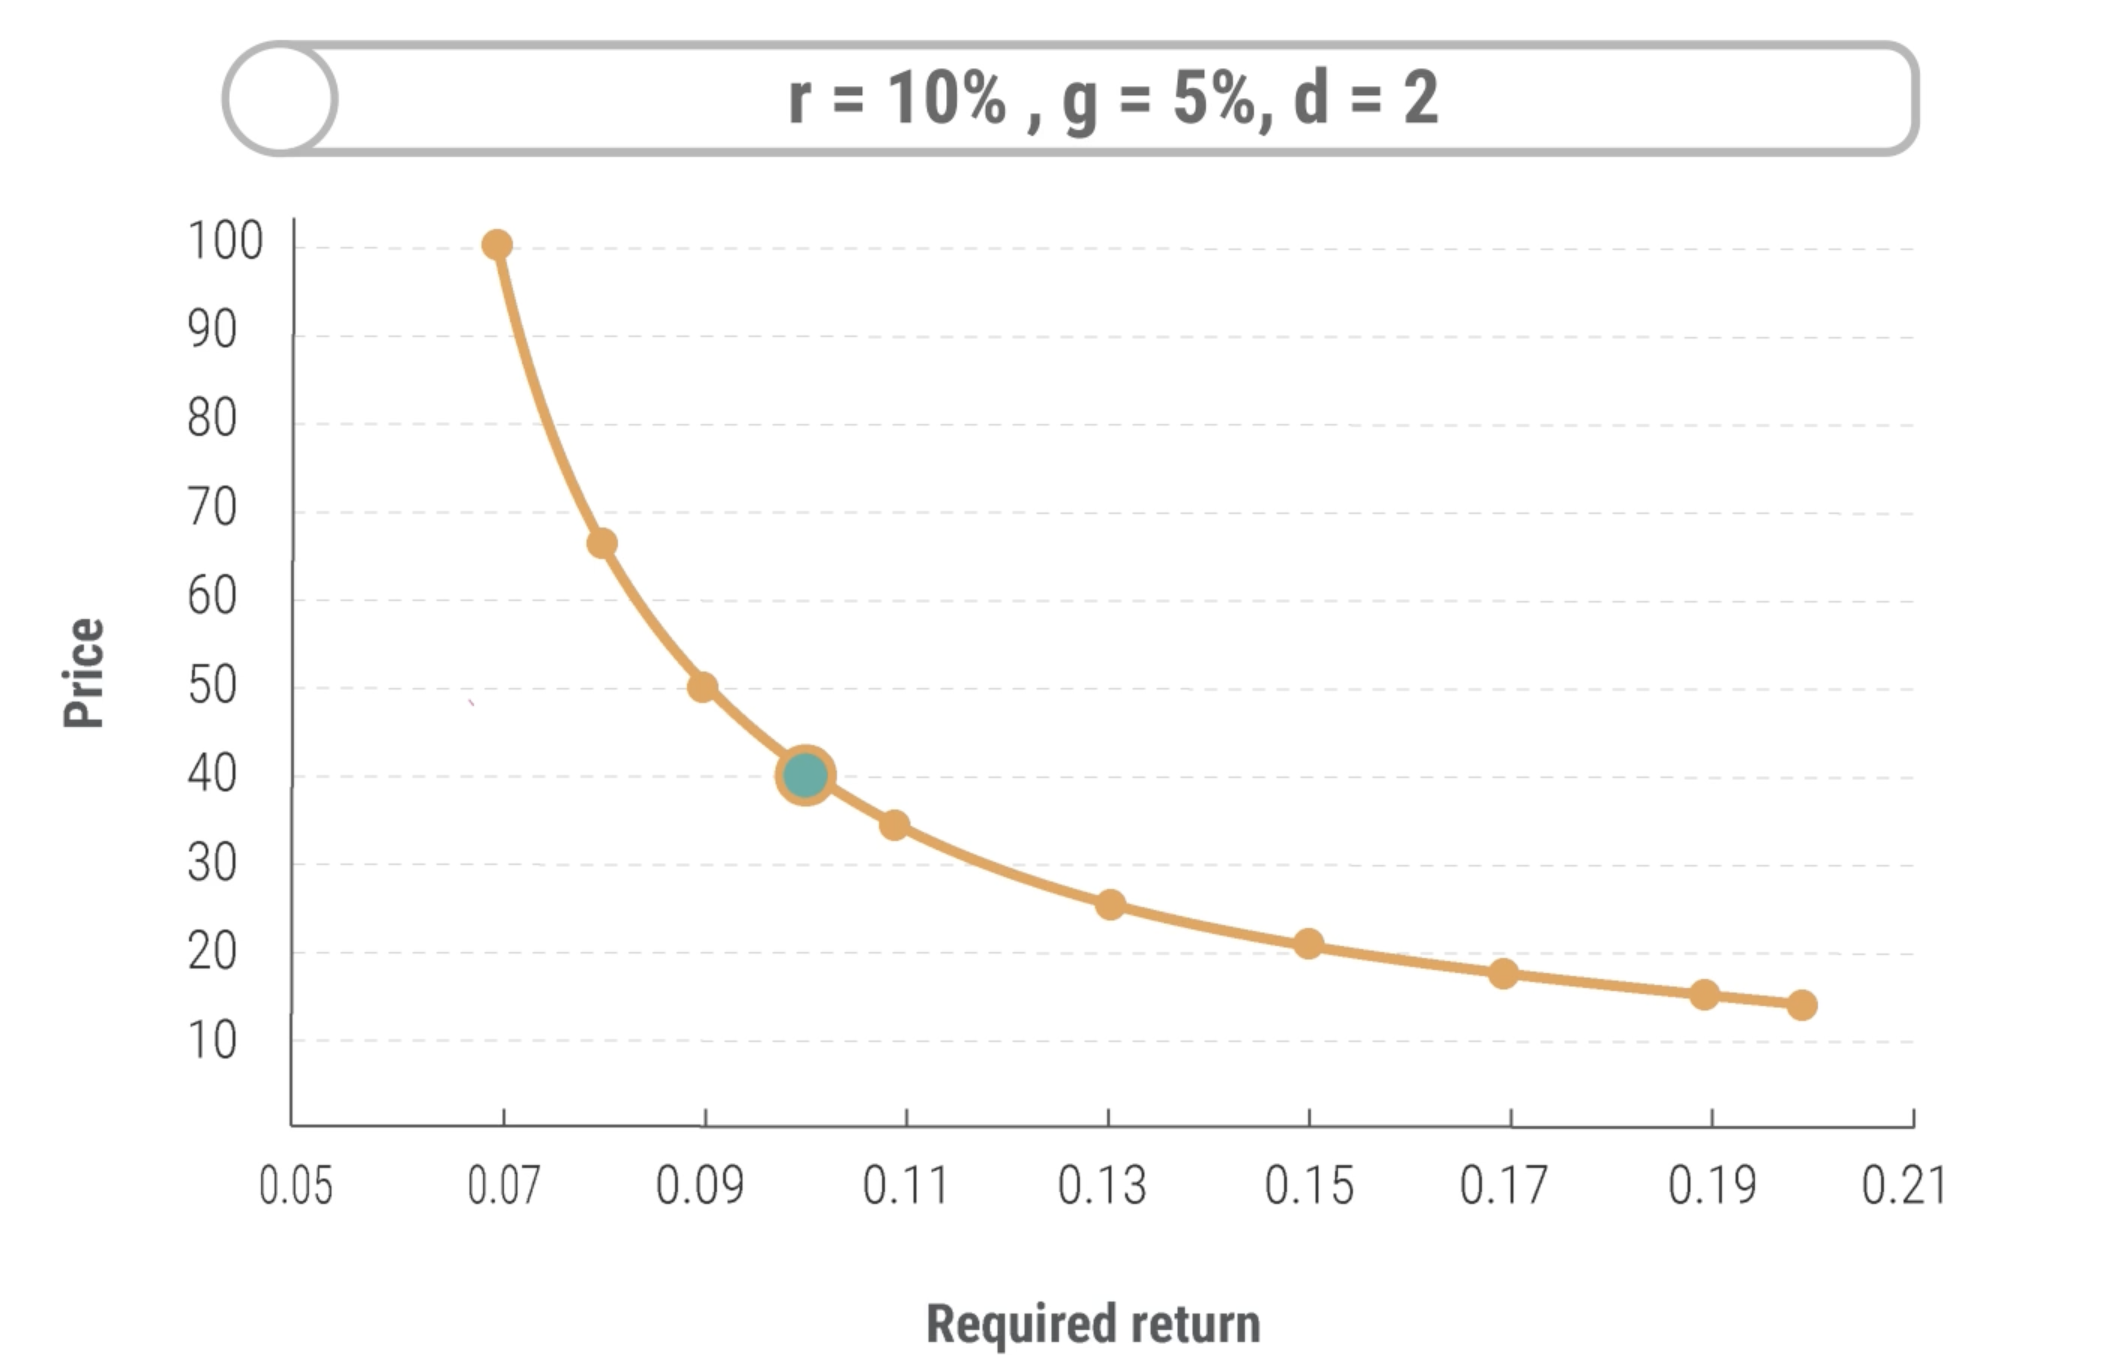
\includegraphics[width=0.5\textwidth]{img/3.4.1.png}
    \end{figure}
    \item Market value is calculated as the dividend $d=2$ divided by the difference between the required rate of return $r$ and the growth rate $g$. So the market value is $2/(0.10-0.05) = 40$.
    \item When there are positive or negative changes in market sentiment, the required rate of return may change, affecting the market value of the stock.
    \begin{figure}[H]
        \centering
        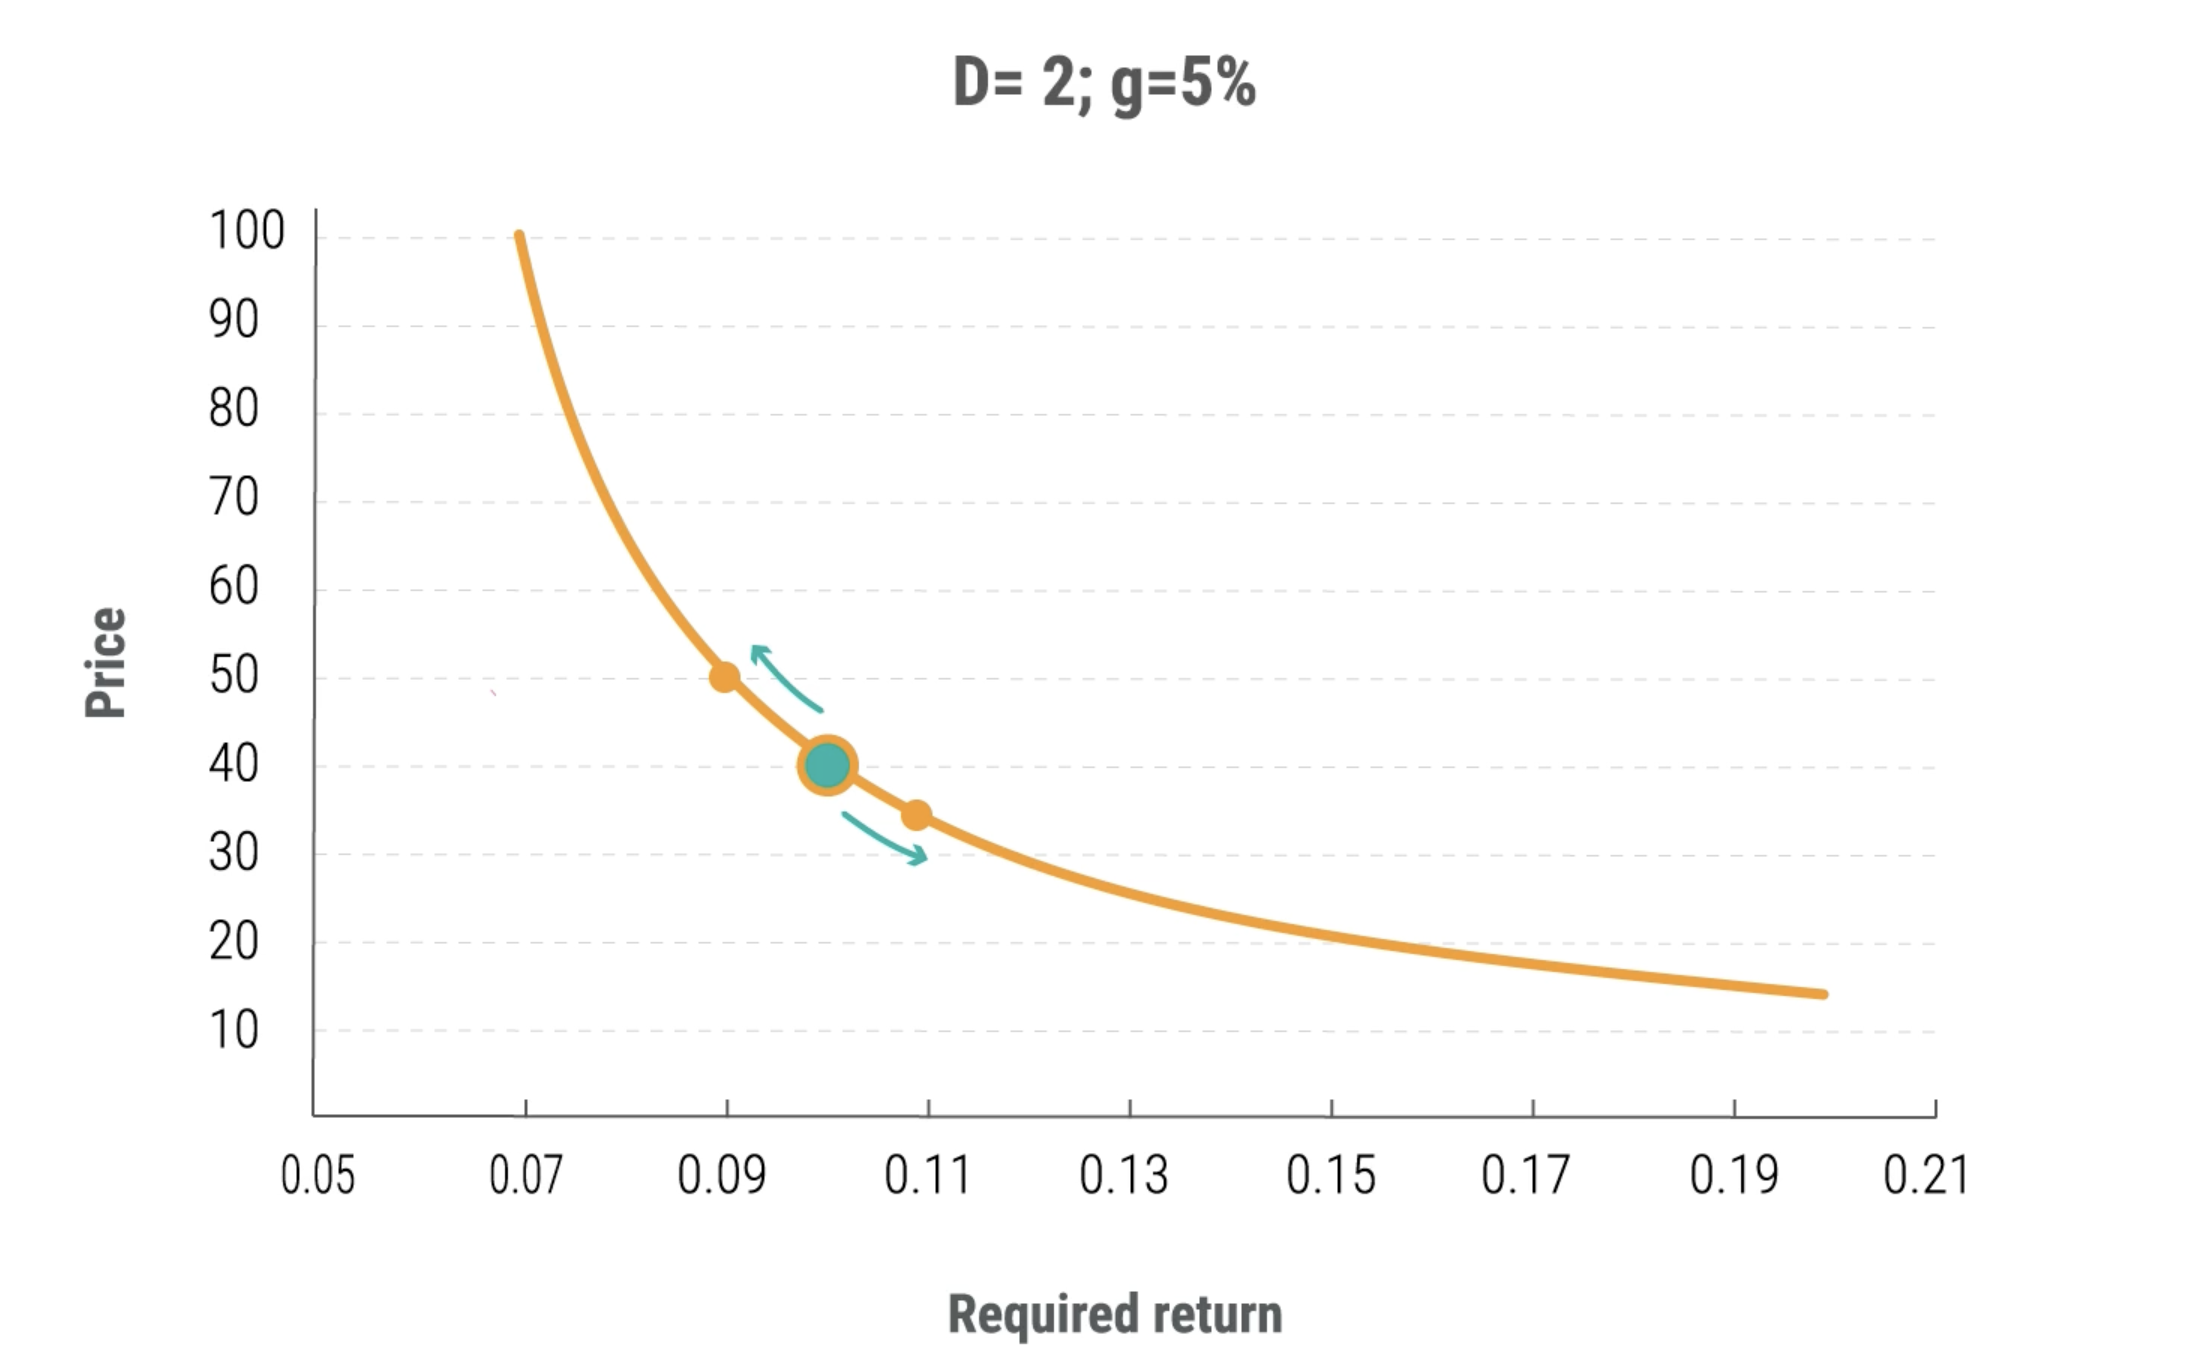
\includegraphics[width=0.5\textwidth]{img/3.4.2.png}
    \end{figure}
    \item A debt crisis may make investors more risk-averse and demand a higher rate of return which then reduces the market value/price of the stock.
    \item On the other hand, a positive economic outlook may reduce the required rate of return, increasing the market value/price of the stock.
    \item This simple model shows why markets can be so sensitive to changes in sentiment and expectations about the future.
    \item Shares are considered to have almost unlimited lifespans, which implies high sensitivity to small changes in the required rate of return, similar to (long-term) bonds that are sensitive to changes in interest rates.
\end{itemize}

We can manipulate the formula to find the required rate of return for a stock given its dividend $Div$, price $P$, and growth rate $g$. The formula is as follows:
\begin{equation}
    r_E = \underbrace{\frac{Div}{P}}_{\text{Dividend Yield} } + \underbrace{g}_{\text{Growth Rate}} 
\end{equation}

\begin{itemize}
    \item Assume that in a given year, the UK market had a dividend yield of 4.5\% and a growth rate of 5\%. Then, the required rate of return for the UK market would be 9.5\%.
\end{itemize}

\section{Case study: Shiller and Siegel}
\textbf{Reading Links:}
\begin{itemize}
    \item \href{https://www.ft.com/content/23c9f650-10c7-11e3-b5e4-00144feabdc0}{Clash of the Cape Crusaders: The world’s leading market historians are locked in an intense debate over the true value of stocks
    }
    \item \href{https://www.advisorperspectives.com/articles/2014/02/18/cape-crusaders-the-shiller-siegel-shootout-at-the-q-group-corral}{A breakdown of their debate}
    
    
\end{itemize}
\textbf{Summary}
\begin{itemize}
    \item \textbf{Robert Shiller} and \textbf{Jeremy Siegel} are two prominent economists with differing views on the stock market performance.
    \item \textcolor{blue}{Shiller, a Nobel laureate, is known for his work on the \textbf{Cyclically Adjusted Price Earnings (CAPE) ratio}, which compares stock prices to average earnings over the past 10 years.}
    \item \textcolor{red}{Siegel, a Wharton professor, is a proponent of the \textbf{efficient market hypothesis}, which posits that stock prices reflect all available information.}
    \item \textcolor{blue}{Shiller argues that the CAPE ratio is a reliable indicator of stock market valuation, suggesting that high ratios predict lower future returns.}
    \item \textcolor{red}{Siegel contends that the CAPE ratio is flawed, as it does not account for changes in accounting standards and the impact of low interest rates on stock prices.}
\end{itemize}

\textbf{Robert Shiller's Perspective (Market Overvalued)}
\begin{itemize}
    \item \textbf{Cyclically Adjusted Price/Earnings (CAPE) Ratio:} Shiller utilises the CAPE ratio, which averages earnings over 10 years to smooth out fluctuations and adjusts for inflation. This method is designed to provide a more stable and historically grounded measure of stock market valuation, indicating when stocks are cyclically high or low.
    \item \textbf{Behavioural Finance Insights:} Shiller, being a proponent of behavioural finance, argues that psychological factors often drive market errors. He believes that the current high readings of the CAPE ratio reflect an overvalued market driven by investor psychology rather than underlying economic fundamentals.
    \item \textbf{Historical Context and Mean Reversion:} Shiller points to historical trends where the CAPE ratio has reverted to the mean after extreme highs, suggesting that periods of high CAPE values are often followed by market corrections or crashes.
\end{itemize}

\textbf{Jeremy Siegel's Perspective (Market Undervalued)}
\begin{itemize}
    \item \textbf{Revised CAPE Ratio:} Siegel has proposed modifications to the CAPE ratio, arguing that changes in accounting practices and economic conditions over time have rendered the traditional CAPE ratio based on Shiller’s model as outdated and pessimistic. Siegel’s adjustments suggest that the market is currently undervalued rather than overvalued.
    \item \textbf{Long-term Stock Market Trends:} Siegel emphasises the historical performance of stocks, noting that over long periods, equities have tended to outperform other asset classes even when adjusted for inflation. This underpins his belief in the "buy-and-hold" strategy, suggesting that fears of overvaluation may be overstated.
    \item \textbf{Optimism about Earnings Growth:} Siegel also points to a trend of increasing earnings growth since World War II, driven by companies retaining more earnings rather than paying them out as dividends. This, he argues, should lead to a higher equilibrium CAPE ratio, implying that the stock market can sustain higher valuation levels without being overvalued.
\end{itemize}

\section{Features of common stock and preferred shares}

Companies may issue multiple classes of stock, which can have different voting rights and privileges.
Common stockholders typically have the right to vote on company matters, while preferred stockholders may not possess voting rights but receive preferential treatment in terms of dividend payments or liquidation proceeds.

Different classes of stock enable companies to offer various rights and benefits to different shareholders. 

\begin{itemize}
    \item \textbf{Voting Rights: }Shares give ownership rights in relation to how the company is run. These rights are invariably exercised through voting at shareholder meetings, e.g. the Annual General Meeting (AGM).
    \item \textbf{Proxy Voting: }Proxy voting is a mechanism where shareholders delegate their voting rights to another party. Historically, fund managers nominated the board of directors as their proxy, but this is now changing, as fund managers want to be more active in matters relating to company decision-making.
    \item \textbf{Classes of Stock: }Some firms have different classes of common stock. These classes often differ in their voting rights — for example, Moller - Maersk has A and B shares, but only class A shareholders have voting rights.
    \item \textbf{Other Rights: }
    \begin{itemize}
        \item The proportion received in declared dividends and/or remaining assets during liquidation. (Some shares get more or less of dividends and liquidated assets)
        \item Pre-emptive rights — the first ‘option to buy’ a new stock issue is offered to existing shareholders
        \item Since 2006, this option-to-buy right has been required by UK law, unless shareholders have actively voted to drop the provision. This is not the case in the USA.
    \end{itemize}
    \item \textbf{Dividend Characteristics: }
    \begin{itemize}
        \item Dividends are not a liability of the firm until they have been declared by the board.
        \item Consequently, a firm cannot go bankrupt for not paying any dividends.
        \item Dividends are paid out of post-tax earnings; they are not tax-deductible.
    \end{itemize}
\end{itemize}


\section{Market Efficiency}

\begin{itemize}
    \item Efficient capital markets are a theoretical model of how financial markets operate under certain conditions, assuming all information is freely available and there are no trading costs.
    \item Market efficiency means that all available information is fully reflected in security prices, making it impossible for investors to consistently earn above-average returns for a given level of risk.
    \item In an efficiently functioning market, securities with equal risk should deliver the same return after adjusting for their respective levels of risk.
    \item Market efficiency is divided into three categories based on the information sets we consider:
    
    \begin{enumerate}
        \item \textbf{Weak Form Efficiency: } 
        \begin{itemize}
            \item Based on historical prices only, implying that past prices are already incorporated into current prices. 
            \item An investor relying solely on this information cannot consistently outperform the market. 
            \item Strategies based on technical analysis or momentum trading, where investors chase past price trends, tend to underperform in this context.
        \end{itemize}

        \item \textbf{Semi-Strong Form Efficiency: } 
        \begin{itemize}
            \item Incorporates all publicly available information, including financial statements, news, accounting data, and other data.
            \item It means that even strategies that incorporate any or a combination of fundamental analysis (accounting information) or price data, find it challenging  to outperform the market.
        \end{itemize}
        \item \textbf{Strong Form Efficiency: }
        \begin{itemize}
            \item In the most idealised scenario, all information (including those mentioned above), both private and public, is factored into market prices. In wallstreetbets lingo, everything is \textit{priced in}.
            \item This is rarely believed in practice, as individuals with inside information can sometimes outperform the market (therefore we cannot assume everyone has access to all information).
            \item What really matters is, thus, whether the market is
            semi-strong efficient or weak form efficient.
        \end{itemize} 
    \end{enumerate}

\end{itemize}


